\section{Visione generale della strategia di verifica}
\subsection{Organizzazione}
Il team \gruppo ~ha deciso di porre al centro di ogni periodo l'attività di verifica in quanto essa certifica la qualità del prodotto. L'attività di verifica sarà continua in tutte le fasi del progetto.\\
Il processo di qualifica accompagnerà tutte le fasi di ciclo di vita del software. Ogni procedura di verifica sarà schedulata attraverso appositi strumenti e i risultati saranno analizzati in questo documento. Tramite il diario delle modifiche è possibile tenere traccia dell'attività di verifica effettuata ed operare delle verifiche circoscritte ai soli cambiamenti.
In particolare le operazioni di controllo verranno istanziate quando il prodotto da analizzare avrà raggiunto uno stato in cui presenti differenze sostanziali rispetto allo stato precedente.
Lo schema che rappresenta l'organizzazione e la pianificazione delle attività di verifica è il \textbf{modello a V}(V-model). Il modello dimostra la relazione tra ogni periodo del ciclo di vita dello sviluppo del software e il suo periodo di \textit{testing}.
\begin{figure} [H]
\centering
     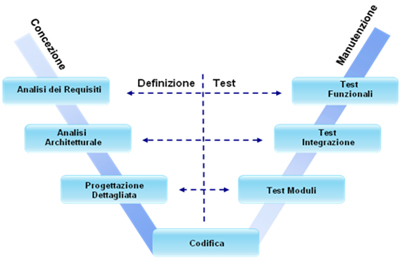
\includegraphics[scale=0.8]{../modello/img/V}\\
     \caption{Modello a V}\label{fig:1}
\end{figure}

L'organizzazione della strategia di verifica prevede l'attività di verifica in tutti i periodi di avanzamento del prodotto, che sono paralleli alle scadenze definite in \infoPDP.
\begin{itemize}
\item \textbf{Analisi}: in questa prima fase il compito del \textit{Verificatore} è innanzitutto relativo alla documentazione e alla correttezza del tracciamento dei requisiti. Ogni documento che servirà per la consegna della RR, una volta ultimata la fase di redazione, verrà verificato in modo definitivo seguendo la procedura così definita:
\begin{enumerate}
\item Verrà controllata la correttezza dei contenuti rispetto alle aspettative del documento tramite una rilettura accurata;
\item Verrà controllata la correttezza grammaticale;
\item Verrà controllato che il documento rispetti le norme definite in \infoNDP ~tramite la lista di controllo presente in tale documento.
\item Verrà verificato che ogni requisito funzionale rilevato abbia una corrispondenza in almeno un caso d'uso e che questo sia tracciato tramite il software di tracciamento che \gruppo ~ha deciso di utilizzare;
\item Verrà verificato che ogni requisito di vincolo e di qualità sia tracciato tramite il software di tracciamento che \gruppo ~ha deciso di utilizzare.
\end{enumerate}
\item \textbf{Progettazione}: il \textit{Verificatore} ha l'importante compito di controllare il soddisfacimento dei requisiti indicati in fase di analisi. Inoltre, si devono verificare che i processi che portano all'incremento dei documenti redatti nel precedente periodo siano conformi alle procedure e regole descritte in \infoNDP;
\item \textbf{Programmazione}: il \textit{Verificatore} provvederà a controlli periodici e pianificati di porzioni di codice, inizialmente di tipo statico per poi passare a dei controlli di tipo dinamico per valutare la correttezza del software;				
\item \textbf{Collaudo}: in questa fase le verifiche saranno esclusivamente di tipo dinamico per garantire che il prodotto risponda a tutti i requisiti indicati e a tutte le richieste del committente: sia implicite che esplicite.
Per le indicazioni precise circa la procedura di verifica adottata dal gruppo si fa riferimento a \infoNDP.
\end{itemize}
Il processo di verifica verterà sulla parte di redazione di documenti, essendo questa un'attività predominante e costante durante tutto il progredire del progetto. Garantendo, altresì che il risultato software sia efficace\ped{G} rispetto alla procedura analizzata, non perdendo di efficienza\ped{G} contrattuale. \\
\subsection{Pianificazione strategica temporale}
Al fine di rispettare in modo ristretto le scadenze citate di seguito e spiegate in modo approfondito in \infoPDP, \gruppo ~ha deciso di pianificare in modo approfondito e sistematico l'attività di verifica. Facendo in modo di rilevare e risolvere nel più breve tempo possibile gli errori che vengono rilevati per evitare che questi possano creare maggiori problematiche nell' avanzamento del prodotto software.\\
Per questo si adottano delle specifiche tecniche in base all'avanzamento del progetto. Ogni attività di redazione dei documenti e di codifica saranno precedute da uno studio preliminare sulla struttura e sui contenuti degli stessi.
\gruppo, conscio della poca esperienza nella pianificazione e gestione di progetti di questo tipo, ha deciso di inserire degli \textit{slack}\ped{G} temporale durante la pianificazione delle attività. Tale scelta è approfondita in \infoNDP ~che ne definisce la quantità e in \infoPDP ~che ne analizza le motivazioni.
L'aggiunta di slack temporali, oltre a portare al progetto una pianificazione più precisa, comporta un aumento dei costi che è però commisurato all'aumento della qualità finale.
\subsection{Obiettivi}
\subsubsection{Qualità di processo}
Al fine di garantire la qualità di prodotto è necessario ricercare la qualità dei processi che lo definiscono. Per questo \gruppo ~ha deciso di adottare lo standard ISO/IEC 15504 denominato SPICE il quale fornisce le indicazioni necessarie a valutare l'idoneità dei processi attualmente in uso.
Per applicare correttamente questo modello, ed adattarlo alla gestione attuata dal gruppo di lavoro, si è deciso di utilizzare il ciclo di Deming o PDCA: il quale definisce una metodologia di controllo dei processi durante il loro ciclo di vita permettendo, inoltre, di migliorare in modo continuo la qualità.
\subsubsection{Qualità di prodotto}
Al fine di aumentare il valore del prodotto e di garantire il corretto funzionamento dello stesso, è necessario fissare degli obiettivi e garantire che questi vengano effettivamente rispettati.
Lo standard ISO/IEC 9126, descritto in appendice A.2, è stato redatto con lo scopo di definire obiettivi e di delineare metriche capaci di misurare il raggiungimento degli stesso.\\
Di seguito elenchiamo le caratteristiche che \gruppo ~si impegna a garantire per il prodotto che andrà a realizzare.
Oltre alla descrizione della caratteristica qui vengono definite le metriche, i parametri di accettazione. 
\begin{itemize}
\item \textbf{Funzionalità}
L’applicazione prodotta deve soddisfare tutti i requisiti obbligatori individuati in \infoAR ~nel modo più completo ed economico possibile, garantendo la sicurezza del prodotto e dei suoi componenti, e adeguandosi alle norme e alle prescrizioni imposte. Inoltre, data la natura del prodotto \progetto, \gruppo ~ha deciso di prestare particolare attenzione al'interoperabilità del codice: intesa come la capacità di agire con altri sistemi.
\begin{itemize}
\item \textbf{misura:} percentuale di requisiti soddisfatti;
\item \textbf{metrica:} la soglia di sufficienza sia il soddisfacimento di tutti i requisiti obbligatori;
\end{itemize}

\item \textbf{Affidabilità}
L’applicazione deve dimostrarsi robusta, di facile ripristino e recupero in caso di errori, e aderire alle norme e alle prescrizioni stabilite.
\begin{itemize}
\item \textbf{misura:} numero di esecuzioni dell'applicazione andate a buon fine;
\item \textbf{metrica:} le esecuzioni dovranno spaziare su tutta la gamma delle possibili casistiche. Il numero di esecuzioni andate a buon fine dovrà essere rapportato al numero totale delle casistiche considerate;
\end{itemize}

\item \textbf{Usabilità}
L’applicazione deve risultare comprensibile, facilmente apprendibile e soprattutto aderire a norme e prescrizioni per garantire facilità d’uso e soddisfacimento delle necessità dell’utente.
\begin{itemize}
\item \textbf{misura:} data l'aleatorietà della qualità richiesta, non si riesce a definire un'unità di misura obiettiva;
\item \textbf{metrica:} non è stata definita una metrica di usabilità; ma \gruppo ~cercherà di offrire la miglior esperienza di utilizzo per tutti coloro che usano il prodotto;
\end{itemize}

\item \textbf{Efficienza}
L’applicazione deve fornire tutte le funzionalità nel minor tempo possibile e con il minimo utilizzo di risorse.
\begin{itemize}
\item \textbf{misura:} il tempo di latenza per ottenere una risposta dal programma;
il tempo di latenza per ottenere una risposta simulando un sovraccarico della rete;
\item \textbf{metrica:} i tempi di latenza dovranno essere in linea con le tempistiche rilevate con l'utilizzo di architetture dello stesso tipo di quelle definite nel prodotto;
\end{itemize}

\item \textbf{Manutenibilità}
L’applicazione deve essere analizzabile, facilmente modificabile e verificabile; inoltre dovrà ridurre il rischio di comportamenti inaspettati al seguito dell'effettuazione di modifiche. Inoltre la documentazione prodotta deve essere chiara e comprensibile.
\begin{itemize}
\item \textbf{misura:} le misurazioni per garantire questa caratteristica sono diverse e non esclusive e sono descritte in seguito;
\item \textbf{metrica:} le metriche da utilizzare sono descritte in seguito;
\end{itemize}

\item \textbf{Portabilità}
L’applicazione deve essere adattabile e compatibile con ambienti d’uso diversi, e con i quali dovrà coesistere condividendo risorse e anche per questo sarà validata da strumenti forniti dal W3C.
\begin{itemize}
\item \textbf{misura:} L'applicazione dovrà essere eseguibile con i browser indicati in \infoAR;
\item \textbf{metrica:} soddisfacimento dei requisiti di compatibilità e validazione tramite strumenti W3C;
\end{itemize}
\end{itemize}
Inoltre, \gruppo ~ ha definito delle altre caratteristi che andranno ricercate per il prodotto:
\begin{itemize}

\item \textbf{Semplicità}: realizzazione del prodotto nella maniera più semplice possibile, ma non semplicistica;
\item \textbf{Incapsulamento}: il codice deve avere visibilità minima e permettere un utilizzo dall’esterno solamente mediante interfacce; ciò aumenta la manutenibilità e la possibilità di riuso del codice;
\item \textbf{Coesione}: le funzionalità che concorrono allo stesso fine devono risiedere nello stesso componente; favorisce semplicità, manutenibilità, riusabilità e riduce l’indice di dipendenza.
\end{itemize}

La definizione delle metriche e gli strumenti utilizzati per la rilevazione delle stesse sono specificate in \infoNDP. Di seguito per ogni metrica indichiamo le misure desiderabili: divise in range ottimale e range di accettazione. D.S indica che sarà definito in seguito.\\
\begin{longtable}{llllXr}
\toprule
\textbf{Metrica} & \textbf{Accettazione} & \textbf{Ottimale}\\
\toprule
SV\ped{1}&$>$-(ore prev x5\%)&$>$0\\
\midrule
BV\ped{2}&$>$-(costo prev x10\%)&$>$0\\
\midrule
Gulpease\ped{3}&40-100&50-100\\
\midrule
Complessità ciclomatica\ped{4}&1-15&1-10\\
\midrule
Livelli di annidamento\ped{5}&1-6&1-3\\
\midrule
Attributi per classe\ped{6}&0-16&3-8\\
\midrule
Parametri per metodo\ped{7}&0-8&0-4\\
\midrule
Linee di codice per &&\\linee di commento\ped{8}&$>$0,25&$>$0,30\\
\midrule
Accoppiamento&D.S.&D.S.\\
\midrule
Copertura&80\%-100\%&85\%-100\%\\
\bottomrule
\caption{parametri delle metriche adottate.}
\end{longtable}

I parametri ottimali e di accettazione sono riferiti a:
\begin{enumerate}
\item Parametro calcolato da \gruppo ~valutando l'inesperienza del gruppo;
\item Parametro calcolato da \gruppo ~valutando l'inesperienza del gruppo;
\item Parametro calcolato in base all'utenza della documentazione;
\item Il valore 10 come massimo fu raccomandato da T.J.McCabe, l'inventore di tale metrica;
\item Valore ideale valutando la chiarezza di codifica;
\item Valore ideale valutando la chiarezza di codifica;
\item Valore ideale valutando la chiarezza di codifica;
\item Il valore 0,30 è ricavato dal rapporto 22/78. Valori ricavati dalle medie dichiarate da Ohlo(Open source network).
\end{enumerate}
\subsection{Procedure di controllo}
\subsubsection{Qualità di processo}
Al fine di garantire la qualità di processo, \gruppo{} adotterà il principio PDCA, descritto nella sezione A.1. Tramite tale tecnica, sarà  garantito un miglioramento continuo dei processi e quindi della qualità degli stessi. Come diretta conseguenza si otterrà il miglioramento qualitativo del prodotto risultante.
Per ottenere questo è necessario che il processo sia in controllo e quindi:
\begin{itemize}
\item Effettuare una dettagliata pianificazione dei processi;
\item Pianificare il numero di risorse da utilizzare, e ripartire le stesse in modo chiaro;
\end{itemize}
Verranno utilizzate due metriche per monitorare la qualità di processo e per mantenere il processo in controllo, queste sono: BV che monitora il il consumo del budget nel tempo e SV che valuta lo stato di avanzamento temporale attuale rispetto a quello pianificato. Le specifiche di queste due metriche sono indicate in \infoNDP. \\
Valori ottimali di BV ed SV indicano un elevato grado di conoscenza ed integrazione del processo come indicato nel CMMI nella sezione A.3.\\
La qualità dei processi viene monitorata inoltre tramite la qualità del prodotto: infatti un prodotto di bassa qualità indica un processo da migliorare.\\
Se su un processo non vengono rilevati problemi, è possibile apportare dei miglioramenti: riducendo il numero di cicli iterattivi, il tempo o le risorse ma garantendo che l'esecuzione del processo sia fedele al piano e soddisfi i requisiti. In questo modo si aumenta l'efficenza del processo e se ne determina un'adattamento positivo alla realtà del team di lavoro valutabile in efficacia.
\subsubsection{Qualità di prodotto}
Il controllo di qualità di prodotto verrà garantito da:
\begin{itemize}
\item \textit{Quality Assurance}: insieme delle attività atte a garantire il raggiungimento degli obiettivi di qualità. Prevede tecniche di analisi statica e dinamica descritte in 2.8;
\item \textit{Verifica}: processo che determina se l'output è consistente, corretto e completo. Il processo di verifica sarà eseguito durante l'intera durata del progetto. I risultati delle attività di verifica saranno riportate in appendice B;
\item \textit{Validazione}: certificazione che attesta la conformità del sistema ai requisiti.
\end{itemize}
\subsection{Risorse umane e responsabilità}
Al fine di garantire l'efficacia e la sistematicità del processo di verifica vengono attribuite delle responsabilità a degli specifici ruoli di progetto.
Per il processo di verifica le responsabilità sono attribuite a \textit{Responsabile di Progetto} ed ai \textit{Verificatori}.
Mentre compito dell' \textit{Amministratore} è quello di supporto a tutte le attività fornendo una solida infrastruttura software anche per il processo di verifica in ogni fase lavorativa.
Per una descrizione più approfondita di ruoli e responsabilità si rimanda a \infoNDP.\\
\subsection{Risorse software}
Al fine di effettuare la fase di verifica e validazione nel modo più sistematico possibile sono stati messi a disposizione di tutti i \textit{Verificatori} dall' \textit{Amministratore} un pacchetto di prodotti software il più specifico possibile rispetto alle esigenze del team. Inoltre, è sempre compito dell' \textit{Amministratore} formare ogni verificatore all'utilizzo dei prodotti che permettano la verifica, evidenziando, se richiesto le funzionalità non utilizzate per ogni prodotto. \gruppo{} ha deciso di adottare questo tipo di formazione per valorizzare il lavoro di chi effettivamente utilizza i prodotti di verifica, dando la possibilità che proprio da queste figure nascano idee e proposte di miglioramento che saranno poi valutate dal \textit{Responsabile di progetto} congiuntamente all'\textit{Amministratore}.
Gli strumenti necessari al raggiungimento degli obiettivi definiti è indicato in \infoNDP, che ne definiscono anche le specifiche tecniche e l'utilizzo.
\subsection{Tecniche di analisi statica}
Questa tecnica di analisi applicabile sia alla documentazione che al codice e permette di effettuare la verifica di quanto prodotto individuando errori ed anomalie. Le tecniche di analisi statica utilizzate sono di tipo \textbf{inspection} per la documentazione, solo a seguito di una prima analisi di tipo \textbf{walkthrough}. Per il codice verrà adottata principalmente una tipologia di analisi \textbf{inspection} per gli errori che sono più ricorrenti o che sono stati rilevati nelle verifiche precedenti.
Per la descrizione si faccia riferimento a \infoNDP.
\subsection{Tecniche di analisi dinamica}
L'analisi dinamica si applica solamente al prodotto software e ciò consiste nell'esecuzione del codice mediante l'uso di test predisposti per verificarne il funzionamento o rilevare possibili difetti di implementazione eseguendo tutto o solo una parte del codice.\\
Al fine di garantire l'utilità del test è necessario che il test sia \textit{ripetibile}. Per \textit{ripetibile} si intende che dato un certo input per la stessa porzione di codice, questo produca sempre lo stesso output sulla stesso ambiente. Per questo motivi saranno definiti a priori:
\begin{itemize}
\item \textbf{Ambiente}: si tratta sia del sistema hardware che di quello software sui quali è stato pianificato l'utilizzo del prodotto; di essi deve essere specificato lo stato iniziale dal quale poter far partire il test;
\item \textbf{Specifica}: definire quali sono gli input e quali dovranno essere gli output attesi;
\item \textbf{Procedure}: definire come sono svolti i test, l'ordine e come devono essere analizzati i risultati;
\end{itemize}
I test verteranno su test di unità per le porzioni di codice prodotte, test di integrazione per le componenti aggiunte in modo incrementale; test di sistema per verificare la corretta esecuzione del sistema; eventuali test di regressione per le modifiche apportate a componenti già testati; e infine test di accettazione per validare il prodotto finale.
\subsubsection{Test di unità}
Verifica di ogni singola unità del prodotto tramite l'utilizzo di stub, driver e logger.
\subsubsection{Test di integrazione}
Verifica dei componenti di sistema che andranno ad incrementare la parte già testata del prodotto; con l'obiettivo di testare la combinazione di più unità garantendone le funzionalità del risultato.
Per l'esecuzione di tali test dovranno essere aggiunte delle componenti fittizie a sostituzione di quelle che non sono ancora state sviluppate, facendo in modo di non influenzare l'esito dell'analisi.
\subsubsection{Test di sistema}
Consiste nella validazione del prodotto software dal momento che lo si ritiene giunto ad una versione definitiva. Tale test ha lo scopo di verificare che la il prodotto copra tutti i requisiti stabiliti in fase di analisi.
\subsubsection{Test di regressione}
Si intende la nuova esecuzione di test a fronte di una modifica di alcune componenti software, per garantire la conformità del sistema post modifica.
\subsubsection{Test di accettazione}
Definito come il collaudo del prodotto. Questo test viene eseguito in presenza del proponente ed in caso di esito positivo si può procedere al rilascio ufficiale del prodotto sviluppato.